\subsection{Theoretical predictions for \texorpdfstring{$\pth$}{pTH} as a function of Higgs boson couplings}


Differential cross sections may be used to constrain physical parameters.
% 
In the case of Higgs boson production via gluon fusion, finite quark mass effects and moderate variations to Higgs boson couplings may manifest themselves through distortions of the $\pth$ spectrum.
% 
We interpret the $\pth$ spectrum for gluon fusion in terms of modifications of the couplings of the Higgs boson using two models: one tailored to heavy quarks and thus sensitive to effects at high $\pt$~\cite{Grazzini:2017szg,Grazzini:2016paz}, and the other considering the effect of lighter quarks in the gluon fusion loop~\cite{Bishara:2016jga}.
% 
The cross section of Higgs boson production in association with top quarks is taken to scale quadratically with $\kappat$.
% 
The other production processes are taken to be independent of these couplings.
% 
The coupling modifiers are described in the context of the $\kappa$-framework~\cite{LHCHXSWG:YR3}:
% 
\begin{linenomath*}
\begin{equation}
\kappa_{i}^{2} = \frac{y_{i}}{y_{i}^{\text{SM}}}\,,
\end{equation}
\end{linenomath*}
% 
where $y_i$ is the Higgs boson coupling to particle $i$.
% 
The SM value of any $\kappa_i$ is equal to 1.


Recent developments in transverse momentum resummation procedures have allowed more accurate calculations of the $\pth$ spectrum when including the effects of lighter quarks on Higgs boson production via gluon fusion~\cite{Banfi:2013eda,Bozzi:2003jy,Becher:2010tm,Monni:2016ktx}.
% 
The $\pth$ spectrum for gluon fusion has been calculated for simultaneous variations of $\kappac$ and $\kappab$~\cite{Bishara:2016jga}, providing a novel approach to constrain these couplings via the $\pth$ spectrum.
% 
We parameterize the variations computed in Ref.~\cite{Bishara:2016jga} with a quadratic polynomial for each bin of the differential production cross section, including an inhomogeneity due to the interference of the top quark loop with that from the bottom and charm quarks in the gluon fusion production loop.
% 
The Higgs boson coupling to the top quark is fixed to its SM value in this model.
% 
The calculations from Ref.~\cite{Bishara:2016jga} are given up to the scale of the Higgs mass, and thus the $\hbb$ channel (for which the lower limit of the $\pth$ spectrum is $350$\GeV) is not used as input for the results obtained with this model.


A second model producing simultaneous variations of $\kappat$, $\cg$, and $\kappab$ by adding dimension-6 operators to the SM Lagrangian has been built in Refs.~\cite{Grazzini:2017szg,Grazzini:2016paz}.
% 
This study employs an analytic resummation performed up to next-to-next-to-leading-logarithmic (NNLL) order in order to obtain the $\pth$ spectrum at next-to-NLO+NNLL accuracy.
% 
The dimension-6 operator whose coefficient is $\cg$ yields a direct coupling of the Higgs field to the gluon field with the same underlying tensor structure as in the heavy-top mass limit.
% 
In the SM, the value of $\cg$ equals 0.
% 
The derivation of $\cg$ is given in Ref.~\cite{Grazzini:2017szg} and the inclusive cross section is given by $\sigma \simeq \left| 12\cg + \kappat \right|^2 \sigma^\text{SM}$.
% 
Two other operators are included to describe modifications of $\kappat$ and $\kappab$.
% 
While the model allows simultaneous variation of all three coupling modifiers, we consider only simultaneous variations of $\kappat$ and $\cg$, and of $\kappat$ and $\kappab$.
% 
The precomputed spectra are taken as input from Ref.~\cite{Grazzini:2017szg} and are parametrized using a quadratic polynomial, neglecting the interference of the bottom and top quarks in the gluon fusion loop.





% img/interpretation/other/varparcomp_kbkc.pdf
% img/interpretation/other/varparcomp_ktcg.pdf
% img/interpretation/other/varparcomp_ktkb.pdf


\begin{figure}[hbtp]
  \begin{center}
    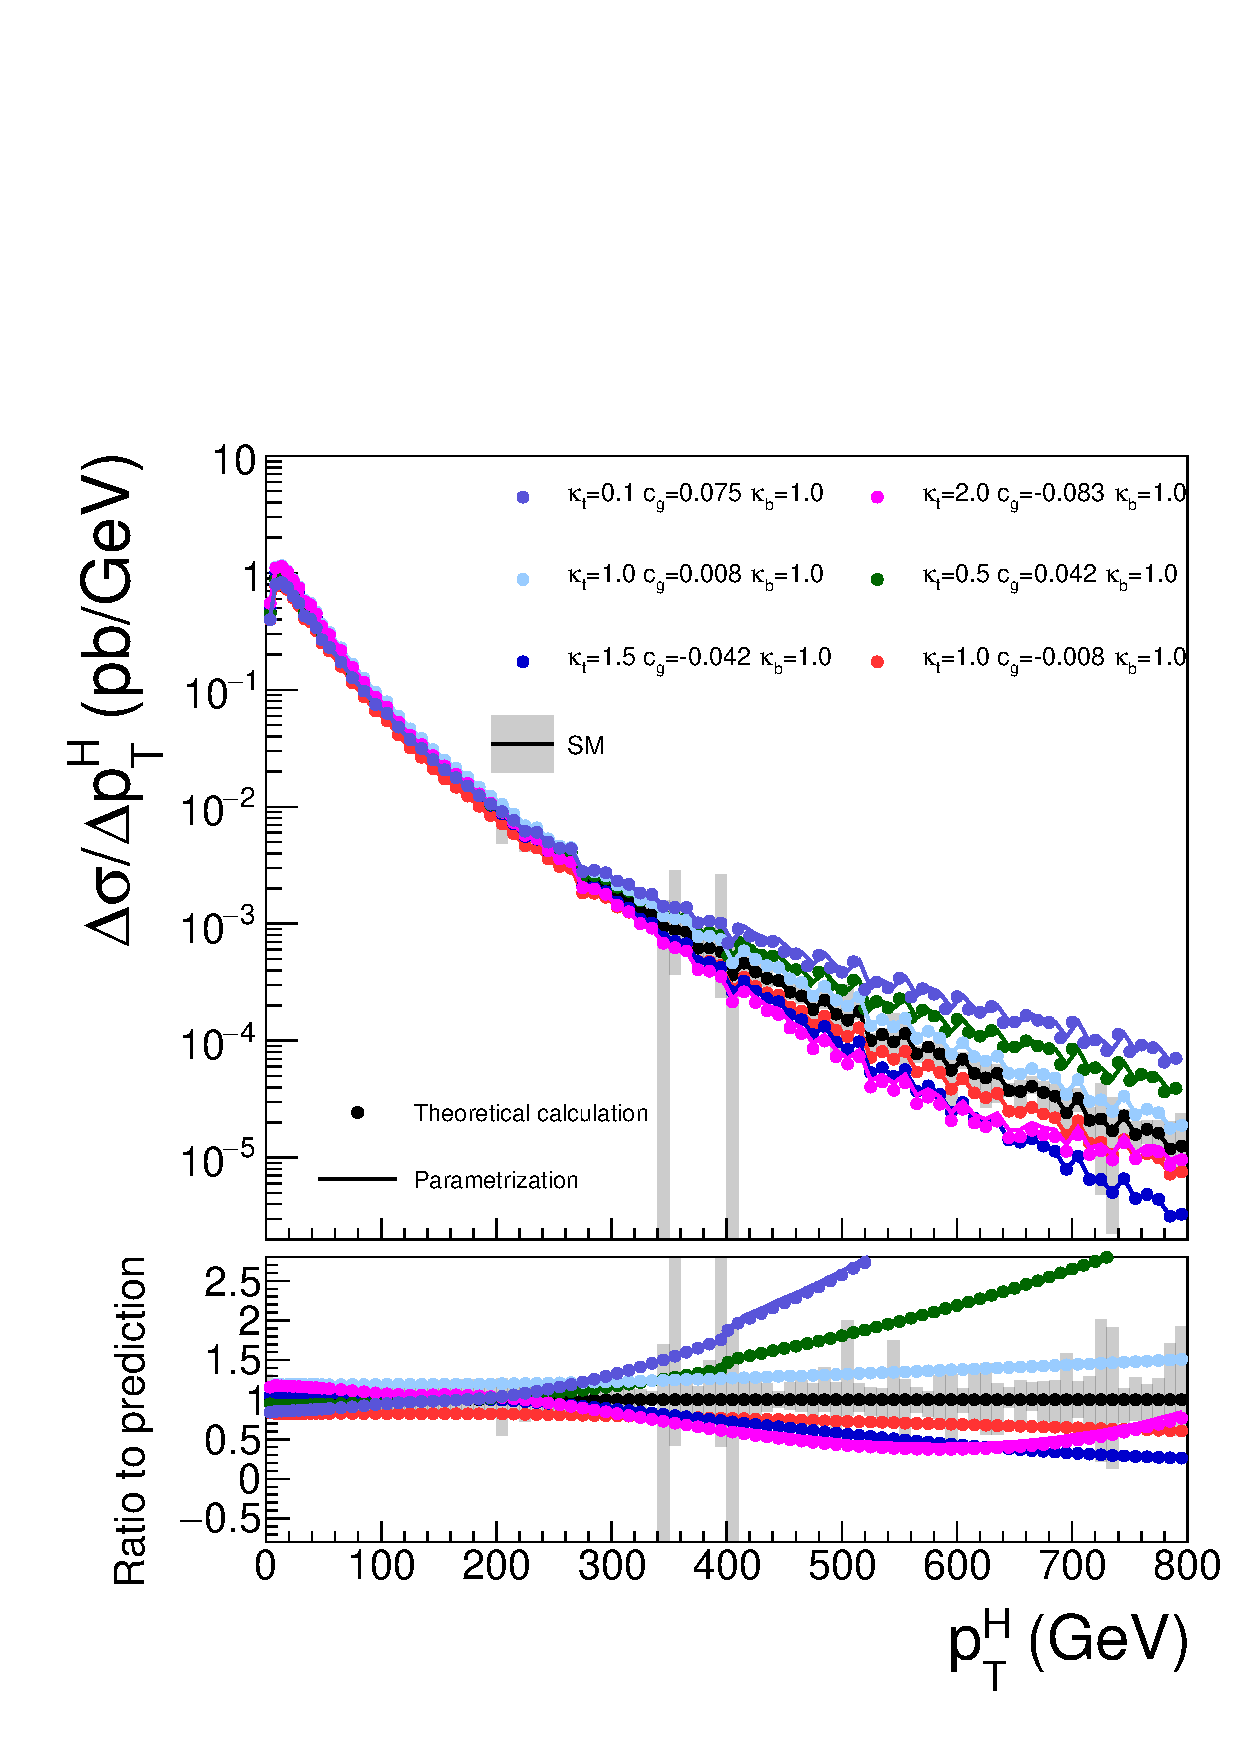
\includegraphics[width=\halflinewidth]{img/interpretation/other/varparcomp_ktcg.pdf}
    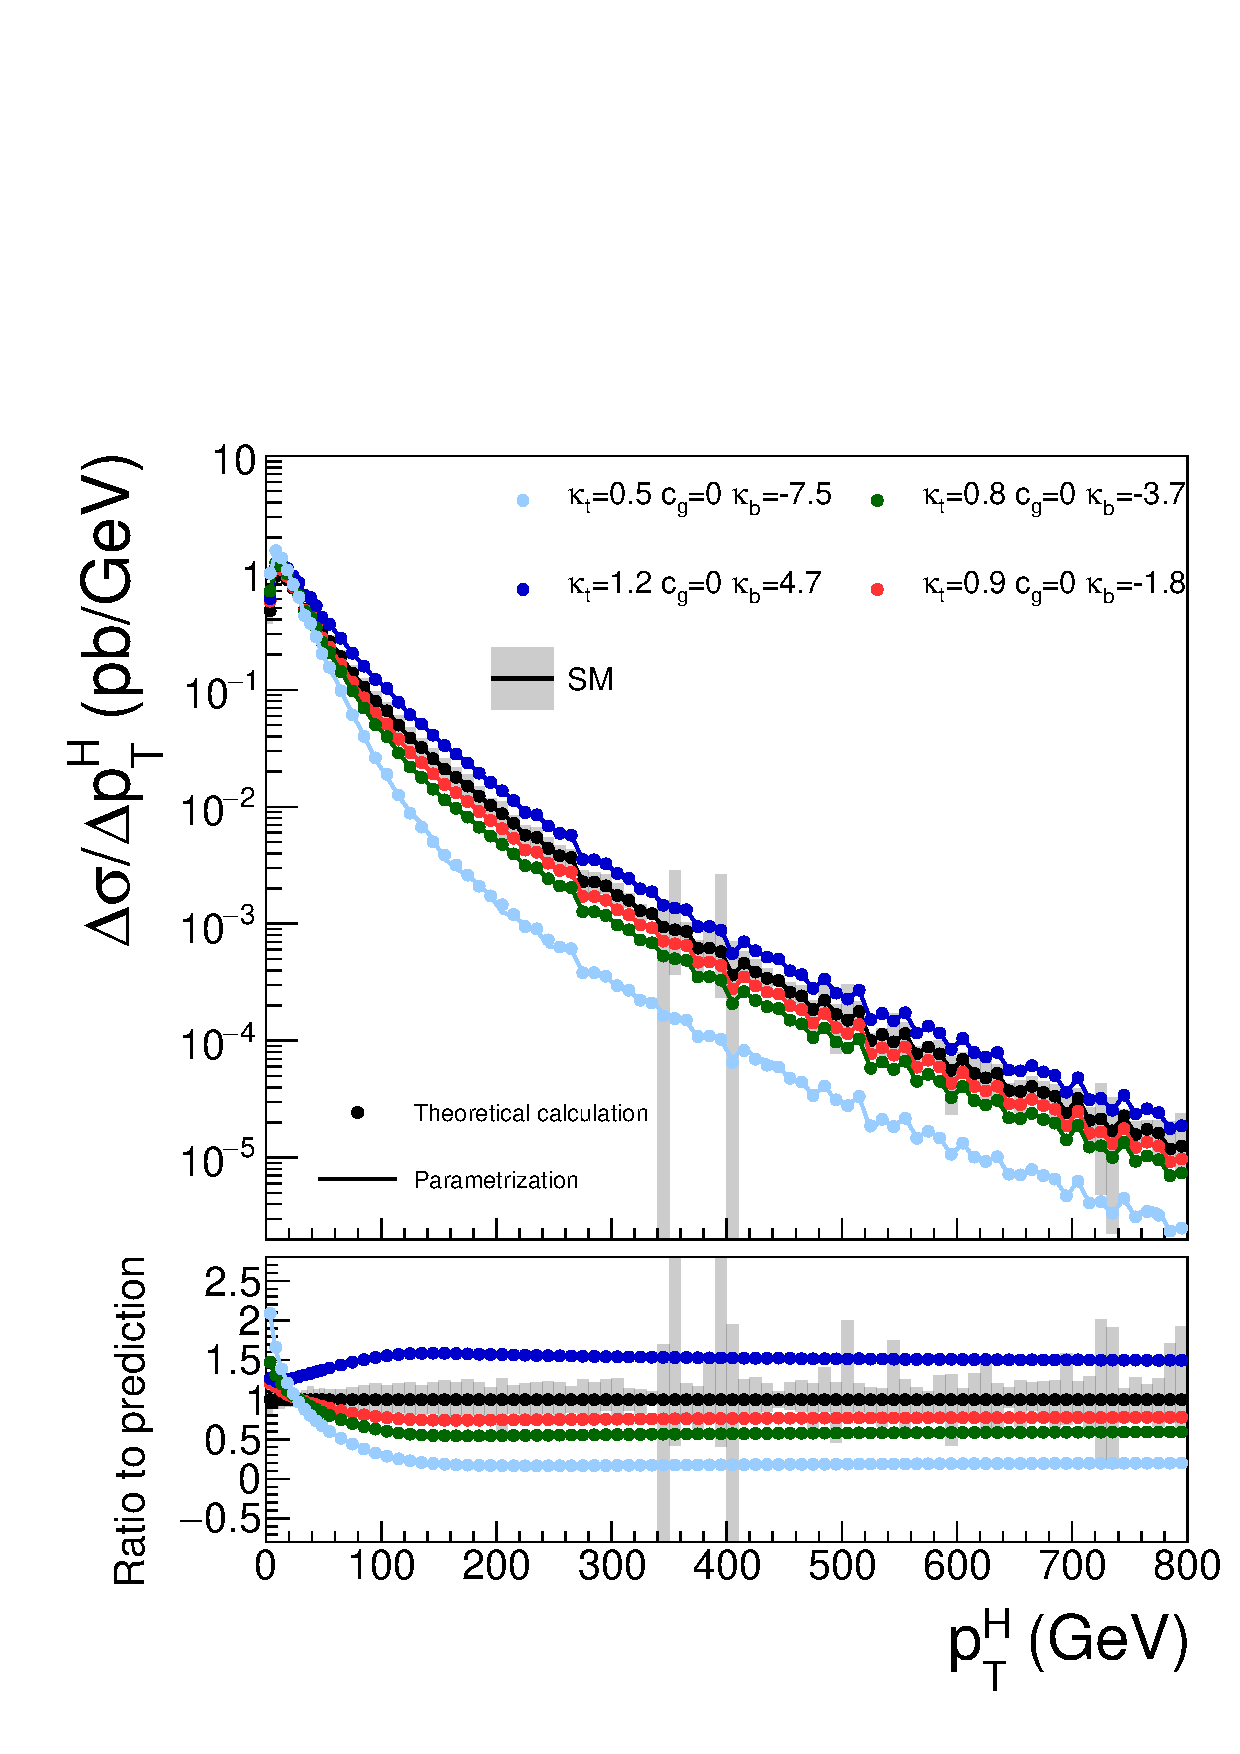
\includegraphics[width=\halflinewidth]{img/interpretation/other/varparcomp_ktkb.pdf}
    % 
    \caption{
        The predicted $\pth$ spectrum for simultaneous variations of $\kappat$ and $\cg$ (left) and $\kappat$ and $\kappab$ (right).
        % 
        The dots correspond to the theoretical calculations performed by the authors in Ref.~\cite{Grazzini:2017szg}, and the corresponding line shows the outcome of the parametrization of the theoretical calculations using a quadratic polynomial.
        % 
        The parametrization matches the exact calculations to a good approximation.
        % 
        The SM prediction is shown in black, with the gray bar indicating the uncertainty due to missing higher order corrections.
        }
    \label{fig:theories_ktcgkb}
  \end{center}
\end{figure}


\begin{figure}[hbtp]
  \begin{center}
    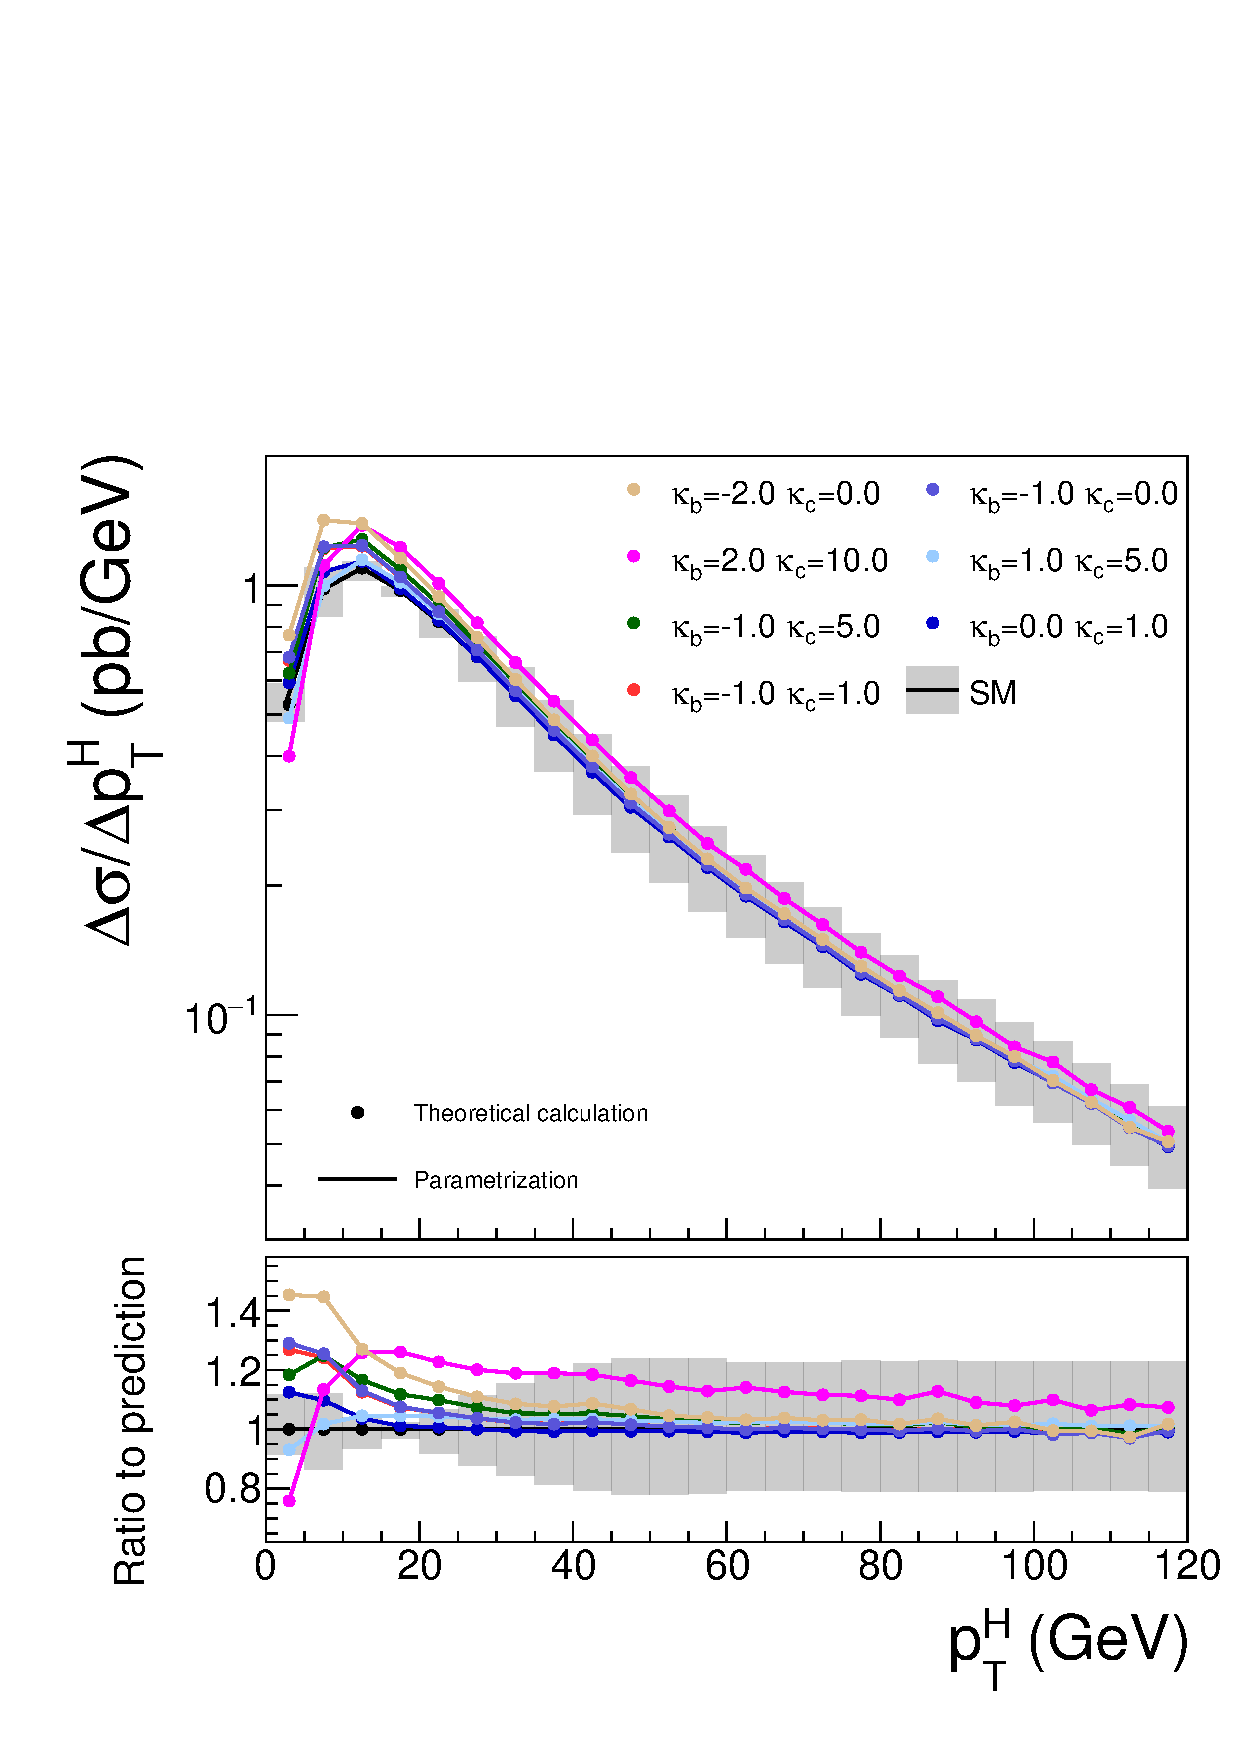
\includegraphics[width=\halflinewidth]{img/interpretation/other/varparcomp_kbkc.pdf}
    % 
    \caption{
        The predicted $\pth$ spectrum for simultaneous variations of $\kappab$ and $\kappac$.
        % 
        The dots correspond to the theoretical calculations performed by the authors in Ref.~\cite{Bishara:2016jga}, and the corresponding line shows the outcome of the parametrization of the theoretical calculations using a fitted quadratic polynomial.
        % 
        The parametrization matches the exact calculations to a good approximation.
        % 
        The SM prediction is shown in black, with the gray bar indicating the uncertainty due to missing higher order corrections.
        }
    \label{fig:theories_kbkc}
  \end{center}
\end{figure}



